%% CUT FROM TAME GOOD STUFF.

We have seen that a system of points and arcs on the unit sphere
can be associated with a centered packing $D$.  The points are the
radial projections of the nodes of $U(D)$ (those at distance at
most $2t_0=2.51$ from the origin).  The arcs are the radial
projections of edges between $v,w\in U(D)$, where $|v-w|\le2t_0$.
If we consider this collection of arcs combinatorially as a
hypermap, then it is not always true that these arcs form a
hypermap in the restrictive sense of
\Chap~\ref{sec:def-and-class}.

The purpose of this \chap\ is to show that if the original
centered packing contravenes, then minor modifications can be made
to the system of arcs hypermap so that the resulting combinatorial
hypermap has the structure of a hypermap in the sense of
\Chap~\ref{sec:def-and-class}. These hypermaps are called
contravening hypermaps.

A natural number $n(R)$ is associated with each standard region. If
the boundary of that region is a simple polygon, then $n(R)$ is the
number of sides.   If the boundary consists of $k$ disjoint simple
polygons, with $n_1,\ldots,n_k$ sides then
    $$n(R) = n_1+\cdots+n_k + 2(k-1).$$

\begin{lemma}\label{cor:std-aggregate-list:bis}
Let $R$ be a standard region in a contravening centered packing
$D$.  The boundary of $R$ is a simple polygon with at most $8$
edges, or one of the configurations of
Figure~\ref{fig:aggregates}.
\end{lemma}

\begin{proof} \shortversion{See \cite{KC}.}
    \longversion{This is Theorem~\ref{thm:the-main-theorem} and
    Corollary~\ref{cor:std-aggregate-list}.}
%Corollary~\ref{cor:std-aggregate-list})
\end{proof}

\begin{figure}[htb]
  \centering
  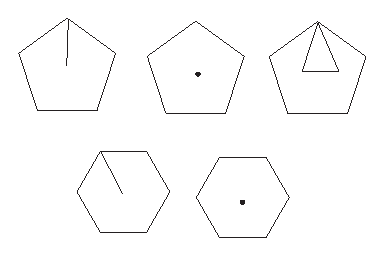
\includegraphics{\ps/nonpolygon.eps}
  \caption{Non-polygonal standard regions ($n(R)=7,7,8,8,8$)}
  \label{fig:aggregates}
\end{figure}

\begin{lemma}\label{lemma:enclosed:bis} % {Lemma 2.2}
A quadrilateral region does not enclose any vertices of height at
most $2t_0$.
\end{lemma}

%% Summation convention:

If $F$ is a face of $H$, let
    $$\sigma_F(D) = \sum \sigma(F),$$
where the sum runs over the set of standard regions associated with
$F$.  This sum reduces to a single term unless $F$ is an aggregate
in the sense of Remarks~\ref{remark:degree6} and
\ref{remark:tri-pent}.


%% Here is stuff for after the definition of formally contravening hypermap.

\begin{assumption}  $H$ is a planar hypermap.  $e$ is an
involution that acts without fixed points.  Every face meets every
node in at most one dart.  Every face has cardinality at least $3$
and at most $8$.
\end{assumption}

%% Here is the stuff for aggregates.

\begin{definition}
The {\it central vertex\/} of a flat quarter is defined to be the
one that does not lie on the triangle formed by the origin and the
diagonal.
%
 \index{central (vertex)}
\end{definition}

\begin{lemma}\label{lemma:1.32:bis}
If the interior angle at a corner $v$ of a non-triangular standard
region is at most $1.32$, then there is a flat quarter over $R$
whose central vertex is $v$.
\end{lemma}

\begin{proof} \shortversion{\cite{KC}.}
    \longversion{This is Lemma~\ref{lemma:1.32}.}
\end{proof}

%% Proof that the hypermap is not empty.

First, we prove the promised non-degeneracy result.

\begin{lemma}
\label{prop:nonempty} The construction of Section
\ref{sec:stargraph} associates a (nonempty) hypermap with at least
two faces to every centered packing $D$ with $\sigma(D)>0$.
\end{lemma}

\begin{proof}
First we show that centered packings with $\sigma(D)>0$ have
nonempty vertex sets $U$. (Recall that $U$ is the set of vertices
of distance at most $2t_0$ from the center).  The vertices of $U$
are used in \Chaps~\ref{sec:construction} and \ref{sec:vcells} to
create all of the structural features of the centered packing:
quasi-regular tetrahedra, quarters, and so forth. If $U$ is empty,
the $V$-cell is a solid containing the ball $B(t_0)$ of radius
$t_0$, and $\sigma(D)$ satisfies
    $$
    \begin{array}{lll}
    \sigma(D) &= \vor(D)\\
              & = -4\doct \op{vol}(\op{VC}(D)) + 4\pi/3 \\
              &< -4\doct\op{vol}(B(t_0)) + 4\pi/3
              &< 0.
    \end{array}
    $$
By hypothesis, $\sigma(D)>0$.  So $U$ is not empty.

Equation~\ref{eqn:sig-all} shows that the function $\sigma$ can be
expressed as a sum of terms $\sigma_R$ indexed by the standard
regions $R$. It is proved in Theorem~\ref{lemma:quad0} that
$\sigma_R\le0$, unless $R$ is a triangle. Thus, a centered packing
with positive $\sigma(D)$ must have at least one triangle. Its
complement contains a second standard region. Even after we form
aggregates of distinct standard regions to form the simplified
hypermap (Remarks \ref{remark:tri-pent} and \ref{remark:degree6}),
there certainly remain at least two faces.
\end{proof}

\section{Contravening Plane Graphs defined}
\label{sec:stargraph}

A hypermap $G$ is attached to every contravening centered packing
as follows.  From the centered packing $D$, it is possible to
determine the coordinates of the set $U(D)$ of vertices at
distance at most $2t_0 $ from the origin.

If we draw a geodesic arc on the unit sphere at the origin with
endpoints at the radial projections of $v_1$ and $v_2$ for every
pair of vertices $v_1$, $v_2\in U(D)$ such that $|v_1|, |v_2|,
|v_1-v_2|\le 2t_0 $, we obtain a hypermap that breaks the unit
sphere into standard regions. (The arcs do not meet except at
endpoints by Lemma~\ref{lemma:2t0-doesnt-pass-through}.)
%Each
%standard region is defined as the closure in the unit sphere of a
%connected component of the unit sphere with all arcs removed.

For a given standard region, we consider the arcs forming its
boundary together with the arcs that are internal to the standard
region.  We consider the points on the unit sphere formed by the
endpoints of the arcs, together with the radial projections to the
unit sphere of vertices in $U$ whose radial projection lies in the
interior of the region.

\begin{remark}
The system of arcs and vertices associated with a standard region in
a contravening example must be a polygon, or one of the
configurations of Figure~\ref{fig:aggregates} (see
Lemma~\ref{cor:std-aggregate-list:bis}).
\end{remark}


\begin{remark} \label{remark:tri-pent}
Observe that one case of Figure~\ref{fig:aggregates} is bounded by a
triangle and a pentagon, and that the others are bounded by a
polygon. Replacing the triangle-pentagon arrangement with the
bounding pentagon and replacing the others with the bounding
polygon, we obtain a partition of the sphere into simple polygons.
Each of these polygons is a single standard region, except in the
triangle-pentagon case (Figure~\ref{fig:tri-pent}), which is a union
of two standard regions (a triangle and a eight-sided region).
\end{remark}
\begin{figure}[htb]
  \centering
  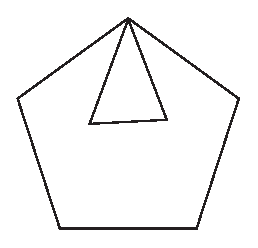
\includegraphics{\ps/tripent.eps}
  \caption{An aggregate forming a pentagon}
  \label{fig:tri-pent}
\end{figure}

\begin{remark}\label{remark:degree6}
To simplify further, if we have an arrangement of six standard
regions around a vertex formed from five triangles and one
pentagon, we replace it with the bounding octagon (or hexagon).
See Figure~\ref{fig:degree6}.  (It will be shown in
Lemma~\ref{lemma:deg5} that there is at most one such
configuration in the standard decomposition of a contravening
centered packing, so we will not worry here about how to treat the
case of two overlapping configurations of this sort.)
\end{remark}
\begin{figure}[htb]
  \centering
  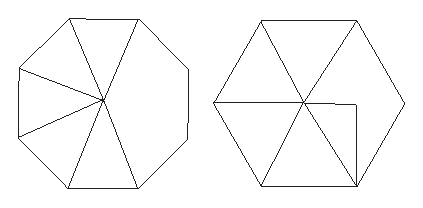
\includegraphics{\ps/degree6.eps}
  \caption{Degree $6$ aggregates}
  \label{fig:degree6}
\end{figure}

In summary, we have a hypermap that is approximately that given by
the standard regions of the centered packing, but simplified to a
bounding polygon when one of the configurations of Remarks
\ref{remark:tri-pent} and \ref{remark:degree6} occur.  We refer to
the combination of standard regions into a single face of the
hypermap as {\it aggregation}.  We call it the hypermap $G = G(D)$
attached to a contravening centered packing $D$.
%
 \index{aggregation}

Lemma~\ref{prop:nonempty} will show the vertex set $U$ is non-empty
and that the hypermap $G(D)$ is non-empty.

When we refer to the hypermap in this manner, we mean the
combinatorial hypermap as opposed to the embedded metric graph on
the unit sphere formed from the system of geodesic arcs.  Given a
node $v$ in $G(D)$, there is a uniquely determined vertex $v(D)$ of
$U(D)$ whose radial projection to the unit sphere determines $v$. We
call $v(D)$ the {\it corner} in $U(D)$ over $v$.
%
 \index{corner}

By construction, the hypermaps associated with a centered packing
do not have loops or multiple joins.  In fact, the edges of $G(D)$
are defined by triangles whose sides vary between lengths $2$ and
$2t_0 $. The angles of such a triangle are strictly less than
$\pi$. This implies that the edges of the metric graph on the unit
sphere always have arc-length strictly less than $\pi$. In
particular, the endpoints are never antipodal.  A loop on the
combinatorial hypermap corresponds to a edge on the metric graph
that is a closed geodesic. A multiple join on the hypermap
corresponds on the metric graph to a pair of points joined by
multiple minimal geodesics, that is, a pair of antipodal points on
the sphere.  By the arc-length constraints on edges in the metric
graph, there are no loops or multiple joins in the combinatorial
hypermap $G(D)$.

%\chapter{The Aggregate Cases}
%    \label{sec:aggregate}

\section{Weight Assignments for Aggregates}

\begin{lemma} The bound $tri(v)>2$ holds if $v$ is a node
of an aggregate face.
\end{lemma}

\begin{proof}
The exceptional region enters into the preceding two proofs in a
purely formal way.  Pentagons enter through the bounds
    $$t_5,\ s_5,\ 1.47\,\pt$$
and angles $1.153$, $1.32$.  Hexagons enter through the bounds
    $$t_6,\ s_6$$
and so forth.  These bounds hold for the aggregate faces.  Hence the
proofs hold for aggregates as well.
\end{proof}

\begin{lemma}
Consider a separated set of nodes $V$ on an aggregated face $F$ as
in Remark \ref{remark:tri-pent}.  The Inequality
\ref{definition:admissible:excess} holds (in the definition of
admissible weight assignments):
    $$\sum_{V\cap F\ne\emptyset} (w(F) -d(\card(F)))
            \ge \sum_{v\in V} a(tri(v)).$$
\end{lemma}

\begin{proof}
We may assume that $tri(v)\in\{3,4\}$.

First consider the aggregate of Remark \ref{remark:tri-pent} of a
triangle and eight-sided region, with pentagonal hull $F$. There
is no other exceptional region in a contravening centered packing
with this aggregate:
    $$t_8 + t_5 > \squander.$$
A separated set of nodes $V$ on $F$ has cardinality at most $2$.
This gives the desired bound $$t_8 > t_5 + 2 (1.5)\,\pt.$$

Next, consider the aggregate of a hexagonal hull with an enclosed
node.  Again, there is no other exceptional face. If there are at
most $k\le 2$ nodes in a separated set, then the result follows from
    $$t_8 > t_6 + k (1.5)\,\pt.$$
There are at most three nodes in $V$ on a hexagon, by the
non-adjacency conditions defining $V$. A node $v$ can be removed
from $V$ if it is not the central node of a flat quarter (Lemma
\ref{lemma:split} and Inequalities~\ref{eqn:tau1.32} and
\ref{eqn:tau-alpha}). If there is an enclosed node $w$, it is
impossible for there to be three nonadjacent nodes, each the central
node of a flat quarter.  In fact, by Lemma~\ref{tarski:node},
any enclosed node must have height greater than $2t_0$.



Finally consider the aggregate of a pentagonal hull with an enclosed
node.  There are at most $k\le2$ nodes in a separated set in $F$.
There is no other exceptional region:
    $$t_7 + t_5 > \squander.$$
The result follows from
    $$t_7 > t_5 + 2(1.5)\,\pt.$$
\end{proof}

\begin{lemma}
Consider a separated set of nodes $V$ on an aggregate face of a
contravening hypermap as in Remark~\ref{remark:degree6}.  The
Inequality~\ref{definition:admissible:excess} holds in the
definition of admissible weight assignments.
\end{lemma}

\begin{proof}
There is at most one exceptional face in the hypermap:
    $$t_8 + t_5 > \squander.$$
Assume first that aggregate face is an octagon (Figure
\ref{fig:degree6}). At each of the nodes of the face that lies on a
triangular standard region in the aggregate, we can remove the node
from $V$ using Lemma \ref {lemma:split} and the estimate
    $$\tauLP(4,0,2\pi-2 (0.8638)) > 1.5\,\pt.$$
This leaves at most one node in $V$, and it lies on a node of $F$
which is ``not aggregated,'' so that there are five standard
regions of the associated centered packing at that node, and one
of those regions is pentagonal.  The value $a(4)=1.5\,\pt$ can be
estimated at this node in the same way it is done for a
non-aggregated case in Section~\ref{sec:tri34}.

Now consider the case of an aggregate face that is a hexagon (Figure
\ref{fig:degree6}).  The argument is the same: we reduce to $V$
containing a single node, and argue that this node can be treated as
in Section~\ref{sec:tri34}.  (Alternatively, use the fact that the
pentagon-triangle combination in this aggregate has been eliminated
by Lemma~\ref{lemma:nobad4}.)
\end{proof}


%% STUFF ABOUT CENTRAL VERTICES, QUARTERS AND SO FORTH.

Recall that the central vertex of a flat quarter is defined to be
the one that does not lie on the triangle formed by the origin and
the diagonal.
%
 \index{central}

%%

XX?  We will say that there is a flat quarter centered at $v$, if
the corner $v'$ over $v$ is the central node of a flat quarter and
that flat quarter lies in the cone over an exceptional region.

%%


%% Table simplified...  The entry (7,0) with 14.76 is relevant here.
%% It needs to be treated.

Define constants $\tlp(p,q)/\pt$ by Table~\ref{eqn:old5.1:bis}. The
entries marked with an asterisk will not be needed.
%
 \index{type (of a node)}
 \index{ZZtauLP@$\tlp(p,q)$}

\begin{equation}
\vbox{\offinterlineskip \hrule
\halign{&\vrule#&\strut\ \hfil#\hfil\ \cr   % "\ " was quad
height 7pt&\omit&&\omit&&\omit&&\omit&&\omit&&\omit&&\omit&\cr
&\hfil $\tlp(p,q)/\pt$\hfil
        &&\hfil $q=0$\hfil
        &&\hfil1\hfil
        &&\hfil2\hfil
        &&\hfil3\hfil
        &&\hfil4\hfil
        &&\hfil5\hfil&
\cr height 7pt&\omit&&\omit&&\omit&&\omit&&\omit&&\omit&&\omit&\cr
\noalign{\hrule}
height7pt&\omit&&\omit&&\omit&&\omit&&\omit&&\omit&&\omit&\cr
&$p=0$&& *&& *&& 15.18&& 7.135&& 10.6497&& 22.27&\cr &1&&    *&& *&&
6.95&& 7.135&&17.62  && 32.3&\cr &2&&    *&&
8.5&&4.756&&12.9814&&*&&*&\cr &3&& *&& 3.6426&&8.334&&20.9&&*&&*&\cr
&4&&4.1396&&3.7812&&16.11&&*&&*&&*&\cr
&5&&0.55&&11.22&&*&&*&&*&&*&\cr &6&&6.339&&*&&*&&*&&*&&*&\cr
&7&&14.76&&*&&*&&*&&*&&*&\cr
height7pt&\omit&&\omit&&\omit&&\omit&&\omit&&\omit&&\omit&\cr}
\hrule }
    %oldtag 5.1
    \label{eqn:old5.1:bis}
\end{equation}


%%  (1,0,1)

\section{A Non-contravening Four-circuit}
\label{sec:impossible-circuit}

This subsection rules out the existence of a particular four-circuit
on a contravening hypermap.  The interior of the circuit consists of
two faces: a triangle and a pentagon.  The circuit and its interior
node are show in Figure~\ref{fig:no4circuit:bis} with nodes marked
$p_1,\ldots,p_5$. The node $p_1$ is the interior node, the triangle
is $(p_1,p_2,p_5)$ and the pentagon is $(p_1,\ldots,p_5)$.


Let $v_1,\ldots,v_4,v_5$ be the corresponding vertices of $U(D)$.
XX?.

The diagonals $\{v_5,v_3\}$ and $\{v_2,v_4\}$ have length at least
$2\sqrt2$ by Lemma~\ref{lemma:2t0-doesnt-pass-through}.  If an
azimuth angle of the  quadrilateral is less than $1.32$, then by
Lemma~\ref{lemma:1.32:bis},  $|v_1-v_3|\le\sqrt{8}$.  Thus, we
assume in the following lemma, that all azimuth angles of the
quadrilateral aggregate are at least $1.32$.

%%

\begin{remark}
We have now fully justified the claim made in
Remark~\ref{remark:degree6}: there is at most one node on six
standard regions, and it is part of an aggregate in such a way that
it does not appear as the node of $H$.
\end{remark}

%%%%%%%%%%%%%%%%%%%%%%

%% AGGREGATE STUFF IN THE PROOF OF \ref{definition:tame:score}
%% Property of Tameness.

We consider three cases for Inequality \ref{eqn:sigma}. In the
first case, assume that the face $F$ corresponds to exactly one
standard region in the centered packing.  XX? In this case,
Inequality \ref{eqn:sigma} follows directly from the bounds of
Lemma~\ref{lemma:sn-tn}:
    $$\sigma(F)\le s_n \le c(n)\,\pt.$$

In the second case, assume we are in the context of a pentagon $F$
formed in Remark~\ref{remark:tri-pent}.  Then, again by
Theorem~\ref{lemma:sn-tn}, we have
$$\sigma(F) \le s_3+s_8\le (c(3)+c(8))\,\pt \le c(5)\,\pt.$$
(Just examine the constants $c(k)$.)

In the third case, we consider the situation of Remark
\ref{remark:degree6}.  The six faces give
$$\sigma(F)\le s_5+\sLP(5,0,2\pi-1.153)< c(8)\,\pt.$$
The constant $1.153$ comes from Lemma~\ref{lemma:0.8638}.


%%%%%%%%%%%%%%%%%%%%%%%%%%%%%
